\documentclass[aspectratio=169, xcolor={table}]{beamer}

\mode<presentation>
{
  \usetheme{NYU}
  \usecolortheme{default}
  \usefonttheme{default}
  \setbeamertemplate{navigation symbols}{}
  \setbeamertemplate{caption}[numbered]
}

\usepackage[english]{babel}
\usepackage[utf8]{inputenc}
\usepackage{booktabs}
\usepackage{tikz}
\usepackage{amsmath, amssymb}
\usepackage{pifont}
\usepackage{url}
\usepackage{colortbl}
\usepackage{appendixnumberbeamer}

\usetikzlibrary{arrows.meta, positioning, fit, patterns}

\definecolor{ssl}{RGB}{90, 35, 140}
\definecolor{sup}{RGB}{180, 45, 45}

\newcommand{\cmark}{\textcolor{ssl}{\ding{51}}}
\newcommand{\xmark}{\textcolor{sup}{\ding{55}}}
\newcommand{\sectiondivider}[1]{%
  \begin{frame}[plain]
    \centering
    \vfill
    {\LARGE \textbf{#1}\par}
    \vfill
  \end{frame}
}

\title[Cross-City SSL for E2E Driving]{Self-Supervised Visual Representations for Cross-City Generalization in End-to-End Autonomous Driving}
\subtitle{Methods, Results, and Mechanisms}
\author[A.\ Hamza]{Ali Hamza}
\institute[NYU Tandon]{%
  Department of Electrical and Computer Engineering \\
  NYU Tandon School of Engineering \\[2pt]
  {\footnotesize Advisor: Prof.\ Anna Choromanska \\
   Committee: Prof.\ Ludovic Righetti, Prof.\ David Fouhey}
}
\date{April 2026}
\titlegraphic{\hfill
\includegraphics[height=1.2cm]{nyu_stacked_color}}

\begin{document}

\section{Introduction}

\begin{frame}
  \titlepage
\end{frame}

\begin{frame}{Outline}
  \begin{enumerate}
    \item Introduction
    \item Background and related work
    \item Methodology
    \item Experiments
    \item Discussion
  \end{enumerate}
\end{frame}

\begin{frame}{Motivation: pooled evaluation obscures geographic transfer}
  \begin{columns}[T]
    \column{0.54\textwidth}
    \begin{itemize}
      \item Published pooled \texttt{navtest} scores are high: TransFuser $83.9\pm0.4$, Latent TransFuser $83.5\pm0.6$, DiffusionDrive $88.1$.
      \item Pooled training and pooled evaluation mix Boston, Pittsburgh, Las Vegas, and Singapore.
      \item Those numbers measure interpolation within a known city mixture, not transfer to an unseen city.
    \end{itemize}
    \column{0.46\textwidth}
    \begin{block}{Question}
      What happens when the training city and the evaluation city are disjoint, and the planner is held fixed while only the image backbone changes?
    \end{block}
  \end{columns}
\end{frame}

\begin{frame}{Open-loop evidence of geographic transfer failure}
  \centering
  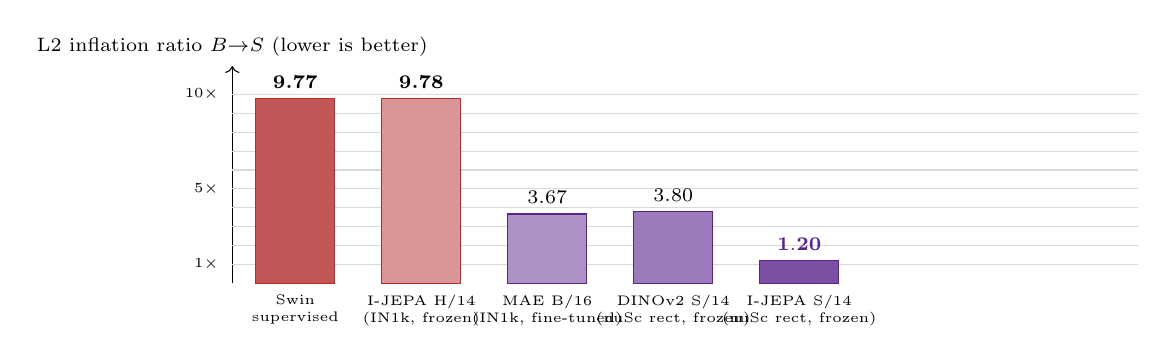
\begin{tikzpicture}[y=0.24cm]
    \draw[->] (0,0) -- (0,11.5) node[above, font=\scriptsize] {L2 inflation ratio $B{\to}S$ (lower is better)};
    \foreach \y in {1,5,10} \node[font=\tiny, anchor=east] at (-0.05,\y) {$\y\times$};
    \foreach \y in {1,2,...,10} \draw[gray!30] (0,\y) -- (11.5,\y);
    \draw[fill=sup!80, draw=sup]  (0.3,0)  rectangle (1.3,9.77);
    \node[font=\scriptsize, anchor=south] at (0.8,9.8) {\textbf{9.77}};
    \node[font=\tiny, anchor=north, align=center] at (0.8,-0.1) {Swin\\supervised};
    \draw[fill=sup!50, draw=sup]  (1.9,0)  rectangle (2.9,9.78);
    \node[font=\scriptsize, anchor=south] at (2.4,9.8) {\textbf{9.78}};
    \node[font=\tiny, anchor=north, align=center] at (2.4,-0.1) {I-JEPA H/14\\(IN1k, frozen)};
    \draw[fill=ssl!50, draw=ssl]  (3.5,0)  rectangle (4.5,3.67);
    \node[font=\scriptsize, anchor=south] at (4.0,3.7) {$3.67$};
    \node[font=\tiny, anchor=north, align=center] at (4.0,-0.1) {MAE B/16\\(IN1k, fine-tuned)};
    \draw[fill=ssl!60, draw=ssl]  (5.1,0)  rectangle (6.1,3.80);
    \node[font=\scriptsize, anchor=south] at (5.6,3.83) {$3.80$};
    \node[font=\tiny, anchor=north, align=center] at (5.6,-0.1) {DINOv2 S/14\\(nuSc rect, frozen)};
    \draw[fill=ssl!80, draw=ssl]  (6.7,0)  rectangle (7.7,1.20);
    \node[font=\scriptsize, anchor=south, text=ssl] at (7.2,1.24) {$\mathbf{1.20}$};
    \node[font=\tiny, anchor=north, align=center] at (7.2,-0.1) {I-JEPA S/14\\(nuSc rect, frozen)};
  \end{tikzpicture}
  \vspace{8pt}
  \begin{itemize}\footnotesize
    \item Boston-to-Singapore open-loop transfer under LAW changes by nearly an order of magnitude when only the image backbone changes.
    \item This is the empirical starting point for the thesis: the visual representation can dominate cross-city failure.
  \end{itemize}
  \footnotesize LAW is treated here as an external baseline cited from earlier joint work.
\end{frame}

\begin{frame}{Central claim}
  \begin{block}{Claim}
    \textbf{Under explicit city-disjoint evaluation, failures in end-to-end driving are strongly mediated by the visual representation. In the evaluated settings, frozen self-supervised backbones transfer more reliably across cities than supervised baselines.}
  \end{block}
  \vspace{6pt}
  \begin{block}{Evidence used in this defence}
    The claim is supported by the lightweight-head study, the LAW benchmark, the completed TransFuser and Latent TransFuser city-disjoint matrices on NAVSIM v1.1, and the full mechanistic analysis. DiffusionDrive is included as a generative-planning extension through pooled results and completed cross-city rows.
  \end{block}
\end{frame}

\begin{frame}{Thesis contributions and study assets}
  \begin{columns}[T]
    \column{0.52\textwidth}
    \textbf{Original work in this thesis}
    \begin{itemize}\footnotesize
      \item City-disjoint evaluation framing and thesis argument.
      \item NAVSIM v1.1 evaluation pipeline and checkpoint re-evaluation.
      \item TransFuser and Latent TransFuser experiments and adapter hardening.
      \item Lightweight-head diagnostic study.
      \item DiffusionDrive integration and analysis.
      \item Mechanistic analysis and synthesis.
    \end{itemize}
    \column{0.48\textwidth}
    \textbf{Inherited assets}
    \begin{itemize}\footnotesize
      \item LAW is an external open-loop baseline.
      \item ImageNet checkpoints are adopted from public releases.
      \item nuScenes SSL checkpoints were produced in collaboration; the domain-specific pretraining pipeline was led by Fatemeh Naeinian.
    \end{itemize}
  \end{columns}
\end{frame}

\section{Background}

\sectiondivider{Background}

\begin{frame}{NAVSIM task and city-disjoint splits}
  \begin{columns}[T]
    \column{0.52\textwidth}
    \textbf{Task definition}
    \begin{itemize}\footnotesize
      \item Inputs: 8 cameras, merged LiDAR, ego state, route.
      \item Output: $8$ future poses over $4$\,s at $2$\,Hz.
      \item Scoring:
      \[
      \mathrm{PDMS} = \mathrm{NC}\!\cdot\!\mathrm{DAC}\!\cdot\!\tfrac{5\,\mathrm{EP}+5\,\mathrm{TTC}+2\,\mathrm{C}}{12}
      \]
      \item NC and DAC are multiplicative. A single severe violation zeros the scenario.
    \end{itemize}
    \column{0.48\textwidth}
    \textbf{City partition}
    \centering
    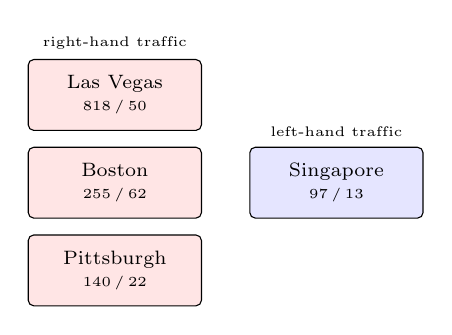
\begin{tikzpicture}[
        city/.style = {draw, rounded corners=2pt, minimum width=22mm, minimum height=9mm, font=\scriptsize, align=center},
      ]
      \node[city, fill=red!10] (lv) {Las Vegas\\{\tiny $818\,/\,50$}};
      \node[city, fill=red!10, below=2mm of lv] (bos) {Boston\\{\tiny $255\,/\,62$}};
      \node[city, fill=red!10, below=2mm of bos] (pit) {Pittsburgh\\{\tiny $140\,/\,22$}};
      \node[city, fill=blue!10, right=6mm of bos] (sg) {Singapore\\{\tiny $97\,/\,13$}};
      \node[font=\tiny, above=0mm of lv] {right-hand traffic};
      \node[font=\tiny, above=0mm of sg] {left-hand traffic};
    \end{tikzpicture}
    \smallskip
    \\{\footnotesize Singapore is the smallest source city and the only left-hand-traffic city.}
  \end{columns}
\end{frame}

\begin{frame}{Mixed-city NAVSIM baselines and internal validation}
  \centering\small
  \begin{tabular}{@{}l c l@{}}
    \toprule
    \textbf{Configuration} & \textbf{PDMS (\%)} & \textbf{Interpretation} \\
    \midrule
    TransFuser, published & $83.9\pm0.4$ & NAVSIM paper mean \\
    Latent TransFuser, published & $83.5\pm0.6$ & NAVSIM paper mean \\
    TransFuser, internal v1.1 & $83.22$ & within published range \\
    Latent TransFuser, internal v1.1 & $83.18$ & within published range \\
    DiffusionDrive, published & $88.1$ & pooled generative reference \\
    \bottomrule
  \end{tabular}
  \vspace{8pt}
  \begin{itemize}\footnotesize
    \item The internal v1.1 TransFuser and Latent TransFuser runs preserve the published ordering and land inside the reported ranges.
    \item All cross-city NAVSIM results in this talk are reported from the canonical thesis matrix under NAVSIM v1.1.
  \end{itemize}
\end{frame}

\section{Related Work}

\sectiondivider{Related Work}

\begin{frame}{Related work and motivating gap}
  \begin{columns}[T]
    \column{0.33\textwidth}
    \textbf{Pooled planner benchmarks}
    \begin{itemize}\footnotesize
      \item Strong leaderboard performance.
      \item Backbone choice is rarely isolated.
      \item Geographic robustness is usually unmeasured.
    \end{itemize}
    \column{0.33\textwidth}
    \textbf{SSL for driving}
    \begin{itemize}\footnotesize
      \item Strong perception and planning results.
      \item Evaluation is often still pooled by geography.
      \item Controlled cross-city planner studies are rare.
    \end{itemize}
    \column{0.33\textwidth}
    \textbf{Cross-city planning}
    \begin{itemize}\footnotesize
      \item Very limited planner-level evidence.
      \item Directional asymmetry is seldom quantified.
      \item Mechanistic evidence is largely missing.
    \end{itemize}
  \end{columns}
  \vspace{6pt}
  \begin{block}{Gap}
    The unresolved question is whether cross-city failure is principally a representation issue once the planner and the training city are controlled.
  \end{block}
\end{frame}

\section{Methodology}

\sectiondivider{Methodology}

\begin{frame}{Experimental design and transfer metrics}
  \textbf{Design principle: hold the planner fixed and vary the image backbone.}
  \smallskip
  \begin{columns}[T]
    \column{0.48\textwidth}
    \textbf{Open-loop transfer ratio}
    \[
      R_{\mathrm{err}}(c_{\mathrm{tr}}\!\to\!c_{\mathrm{te}})
      = \frac{E_{\mathrm{cross}}(c_{\mathrm{tr}}\!\to\!c_{\mathrm{te}})}{E_{\mathrm{in}}(c_{\mathrm{tr}}\!\to\!c_{\mathrm{tr}})}
    \]
    Lower is better. A value of $1$ means perfect retention.
    \column{0.48\textwidth}
    \textbf{Closed-loop out-of-distribution PDMS}
    \[
      S_{\mathrm{OOD}}(c_i)
      = \tfrac{1}{|\mathcal{C}|-1}\sum_{c_j\neq c_i} S(c_i{\to}c_j)
    \]
    Higher is better. Read together with the full $4\times4$ transfer matrix.
  \end{columns}
  \vspace{8pt}
  \footnotesize One model is trained per source city and then evaluated on every destination city without adaptation. All TF and LatTF rows share the same backbone interface and adapter pathway.
\end{frame}

\begin{frame}{Backbone families and planner families}
  \begin{columns}[T]
    \column{0.54\textwidth}
    \textbf{Backbone families}
    \begin{itemize}\footnotesize
      \item Supervised baseline: Swin-T for LAW, ResNet-34 for TF, LatTF, and DiffusionDrive.
      \item SSL objectives: I-JEPA, DINOv2, MAE.
      \item Initialisation sources: ImageNet releases and domain-specific nuScenes ViT-S/14 checkpoints.
      \item Frozen and fully trainable variants are evaluated where applicable.
    \end{itemize}
    \column{0.46\textwidth}
    \textbf{Planner families}
    \begin{itemize}\footnotesize
      \item LAW, open-loop, nuScenes.
      \item TransFuser, closed-loop, camera plus LiDAR.
      \item Latent TransFuser, closed-loop, camera only.
      \item DiffusionDrive, generative planner with anchor trajectories and two-step denoising.
    \end{itemize}
  \end{columns}
\end{frame}

\section{Experiments}

\sectiondivider{Experiments}

\begin{frame}{Study I: lightweight-head design}
  \begin{itemize}
    \item Front camera only, 2-layer MLP trajectory head, $L_1$ loss.
    \item Planner capacity is intentionally minimal, so any PDMS spread is primarily a representation spread.
    \item 45 runs under a shared configuration: 11 backbones, frozen and trainable variants.
  \end{itemize}
  \vspace{6pt}
  \begin{block}{Purpose}
    This study asks whether the representation signal is already visible before introducing a strong planner.
  \end{block}
\end{frame}

\begin{frame}{Study I: pooled lightweight-head results}
  \centering\scriptsize
  \begin{tabular}{@{}l l c@{}}
    \toprule
    \textbf{Backbone} & \textbf{Pre-training} & \textbf{PDMS (\%)} \\
    \midrule
    \textcolor{ssl}{I-JEPA ViT-H/14}  & ImageNet-1k SSL            & $\mathbf{79.7}$ \\
    MAE ViT-B/16                       & ImageNet-1k SSL            & $77.5$ \\
    MAE ViT-S/14                       & nuScenes $224^{2}$         & $74.9$ \\
    MAE ViT-S/14                       & nuScenes $224{\times}392$  & $73.8$ \\
    I-JEPA ViT-S/14                    & nuScenes $224^{2}$         & $71.6$ \\
    DINOv2 ViT-S/14                    & nuScenes $224{\times}392$  & $69.8$ \\
    DINOv2 ViT-S/14                    & nuScenes $224^{2}$         & $69.7$ \\
    \rowcolor{gray!12}
    \textcolor{sup}{ResNet-34}         & ImageNet supervised        & $68.7$ \\
    DINOv2 ViT-S/14                    & LVD-142M SSL               & $66.8$ \\
    I-JEPA ViT-S/14                    & nuScenes $224{\times}392$  & $65.4$ \\
    \bottomrule
  \end{tabular}
  \vspace{8pt}
  \begin{itemize}\footnotesize
    \item Frozen I-JEPA ViT-H/14 leads at $79.7$ PDMS.
    \item Seven of nine frozen SSL variants exceed the supervised ResNet-34 baseline at the same head.
  \end{itemize}
\end{frame}

\begin{frame}{Study I: city-disjoint lightweight-head results}
  \centering\small
  \begin{tabular}{@{}lcccc@{}}
    \toprule
    \textbf{Train city} & \textcolor{sup}{\textbf{ResNet-34}} & DINOv2 & \textcolor{ssl}{\textbf{I-JEPA}} & MAE \\
    \midrule
    Boston     & $61.1$ & $59.8$ & $\mathbf{68.8}$ & $65.4$ \\
    Pittsburgh & $55.6$ & $55.7$ & $\mathbf{65.2}$ & $61.3$ \\
    Las Vegas  & $62.3$ & $59.5$ & $\mathbf{72.2}$ & $69.2$ \\
    Singapore  & $51.1$ & $50.9$ & $\mathbf{52.9}$ & $52.8$ \\
    \midrule
    \rowcolor{gray!12}
    Mean (4 cities) & $57.5$ & $56.4$ & $\mathbf{64.8}$ & $62.2$ \\
    \bottomrule
  \end{tabular}
  \vspace{8pt}
  \begin{itemize}\footnotesize
    \item I-JEPA leads the four-city mean by $+7.3$ points over supervised ResNet-34.
    \item The Singapore row compresses all backbones toward the bottom, which foreshadows the full benchmark.
  \end{itemize}
\end{frame}

\begin{frame}{Study II: cross-city benchmark design}
  \begin{columns}[T]
    \column{0.5\textwidth}
    \textbf{Open-loop benchmark}
    \begin{itemize}\footnotesize
      \item LAW on nuScenes.
      \item Boston and Singapore transfer in both directions.
      \item Identical planner and training recipe across backbones.
    \end{itemize}
    \medskip
    \textbf{Closed-loop benchmark}
    \begin{itemize}\footnotesize
      \item TransFuser and Latent TransFuser on NAVSIM.
      \item Full $4\times4$ training-city by evaluation-city matrix.
      \item All results in this talk come from the canonical thesis matrix under NAVSIM v1.1.
    \end{itemize}
    \column{0.5\textwidth}
    \textbf{Backbone roster}
    \begin{itemize}\footnotesize
      \item Supervised defaults plus ImageNet SSL and nuScenes SSL checkpoints.
      \item Frozen and fully trainable variants where available.
      \item Exact backbone swaps under the same planner are the core controlled comparison.
    \end{itemize}
  \end{columns}
  \vspace{6pt}
  \footnotesize LAW is included as an external baseline. The NAVSIM experiments, re-evaluations, and interpretations are thesis results.
\end{frame}

\begin{frame}{Study IIa: LAW transfer from Boston to Singapore}
  \centering\small
  \begin{tabular}{@{}l c c@{}}
    \toprule
    \textbf{Backbone (LAW)} & $R_\text{L2}$ & $R_\text{coll}$ \\
    \midrule
    \rowcolor{gray!10}
    \textcolor{sup}{Swin-T (supervised, LAW default)} & $\mathbf{9.77\times}$ & $\mathbf{19.34\times}$ \\
    I-JEPA ViT-H/14 (IN1k, frozen)      & $9.78\times$ & $5.18\times$ \\
    MAE ViT-B/16 (IN1k, fine-tuned)     & $3.67\times$ & $10.38\times$ \\
    DINOv2 ViT-S/14 (nuSc rect, frozen) & $3.80\times$ & $7.64\times$ \\
    \textcolor{ssl}{I-JEPA ViT-S/14 (nuSc rect, frozen)} & \textcolor{ssl}{$\mathbf{1.20\times}$} & \textcolor{ssl}{$\mathbf{0.75\times}$} \\
    \bottomrule
  \end{tabular}
  \vspace{8pt}
  \begin{itemize}\footnotesize
    \item With the planner fixed, the representation alone changes the Boston-to-Singapore transfer ratio from $9.77\times$ to $1.20\times$.
    \item The collision ratio also improves from $19.34\times$ to $0.75\times$.
  \end{itemize}
\end{frame}

\begin{frame}{Study IIb: TransFuser cross-city transfer}
  \centering
  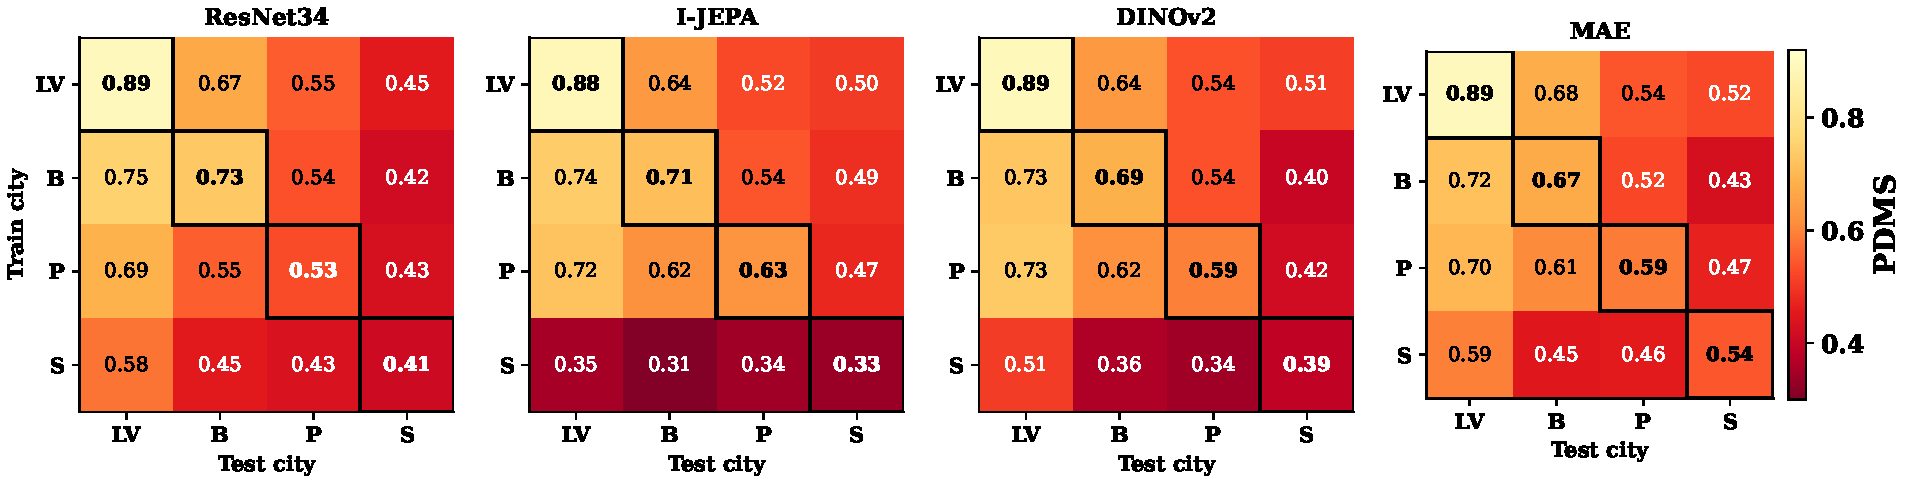
\includegraphics[width=0.96\textwidth]{../fig/iros/fig1_tf_pdms_heatmaps.pdf}
  \vspace{4pt}
  \begin{itemize}\footnotesize
    \item Rows are training cities and columns are evaluation cities.
    \item Singapore is consistently the hardest destination column, and frozen SSL rows improve off-diagonal stability.
  \end{itemize}
\end{frame}

\begin{frame}{Study IIc: Latent TransFuser cross-city transfer}
  \centering
  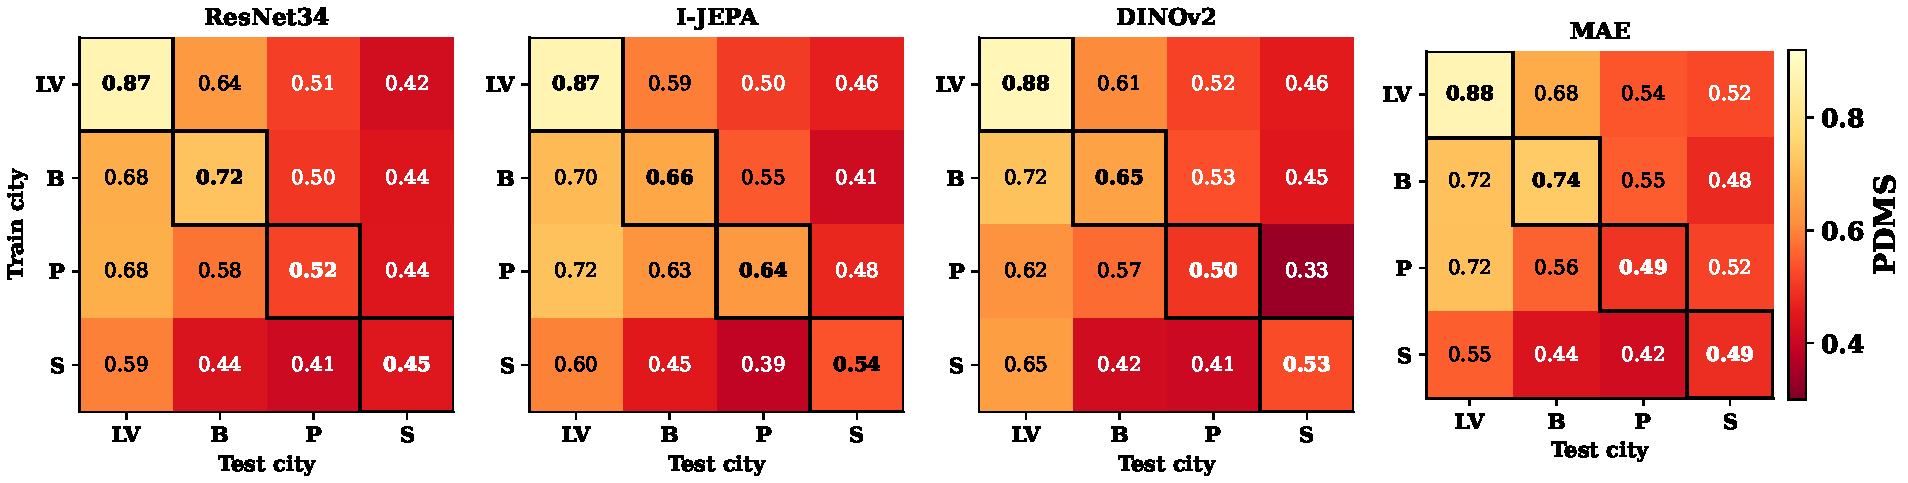
\includegraphics[width=0.96\textwidth]{../fig/iros/fig1_latf_pdms_heatmaps.pdf}
  \vspace{4pt}
  \begin{itemize}\footnotesize
    \item The same cross-city structure appears in the camera-only planner.
    \item The representation effect remains visible without the LiDAR branch.
  \end{itemize}
\end{frame}

\begin{frame}{Cross-city NAVSIM: in-distribution and OOD performance}
  \centering
  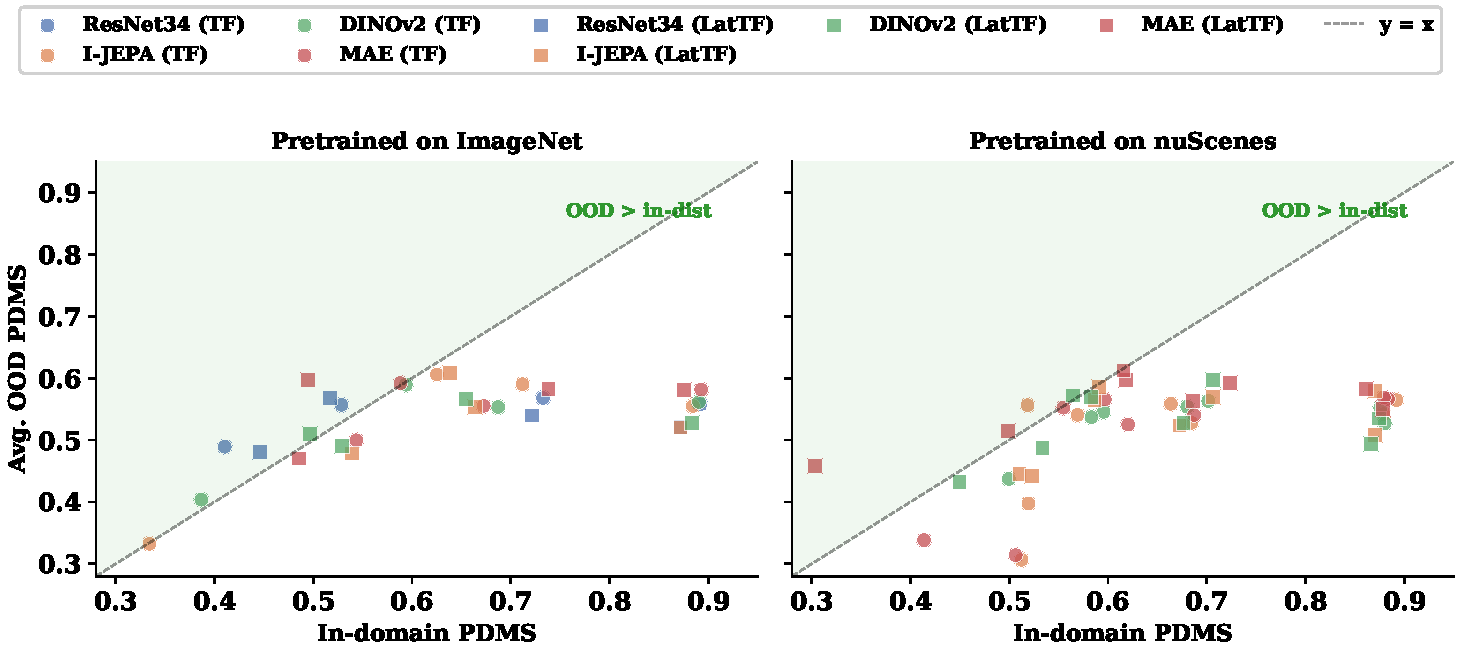
\includegraphics[width=0.82\textwidth]{../fig/iros/fig3_indomain_vs_ood.pdf}
  \vspace{4pt}
  \begin{itemize}\footnotesize
    \item Each point is one trained model; points on the diagonal would transfer without loss.
    \item Supervised rows sit furthest below the diagonal, while the strongest frozen SSL rows stay closer to it.
  \end{itemize}
\end{frame}

\begin{frame}{Cross-city NAVSIM: source-city effects}
  \centering
  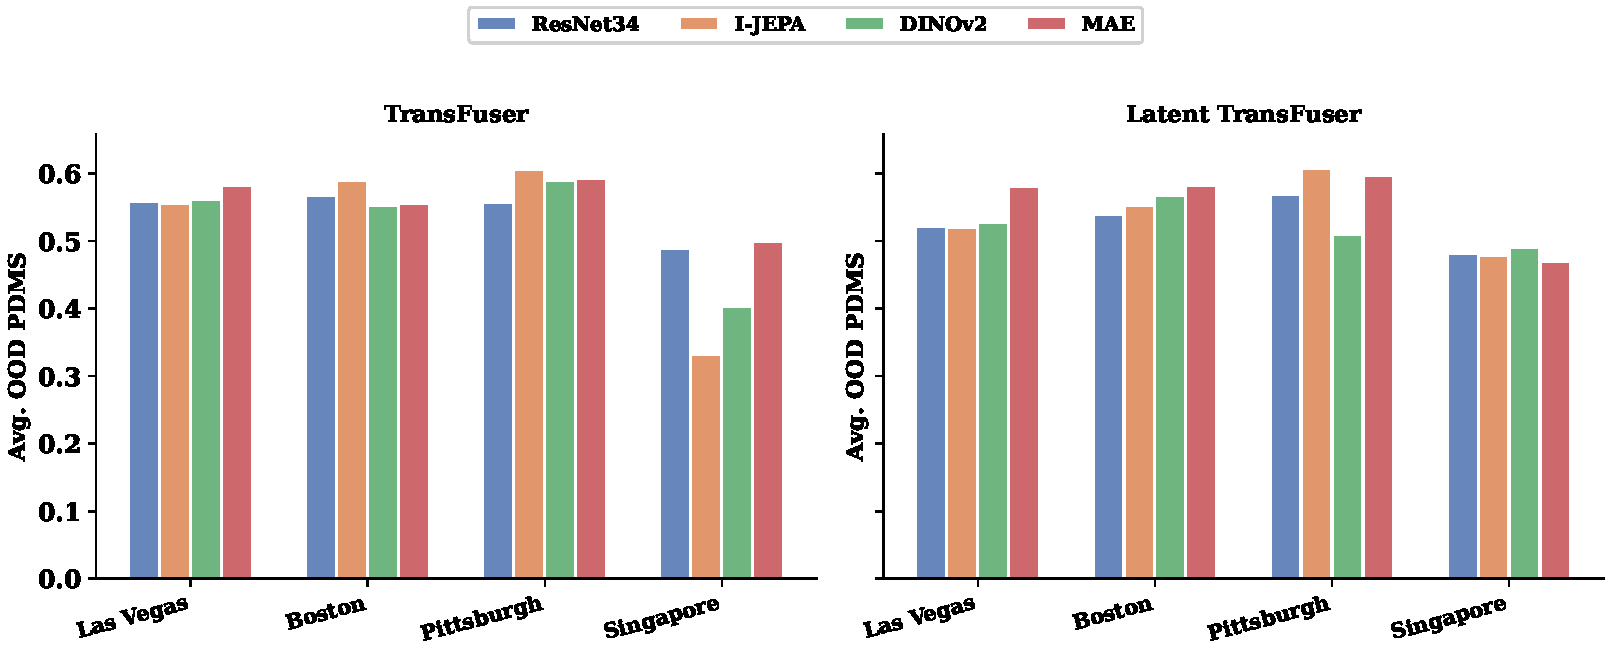
\includegraphics[width=0.82\textwidth]{../fig/iros/fig6_best_training_city.pdf}
  \vspace{4pt}
  \begin{itemize}\footnotesize
    \item Boston and Las Vegas are the strongest training sources across planners and backbones.
    \item Singapore is consistently the weakest source city in the completed matrix.
  \end{itemize}
\end{frame}

\begin{frame}{Cross-city NAVSIM: directional asymmetry}
  \centering
  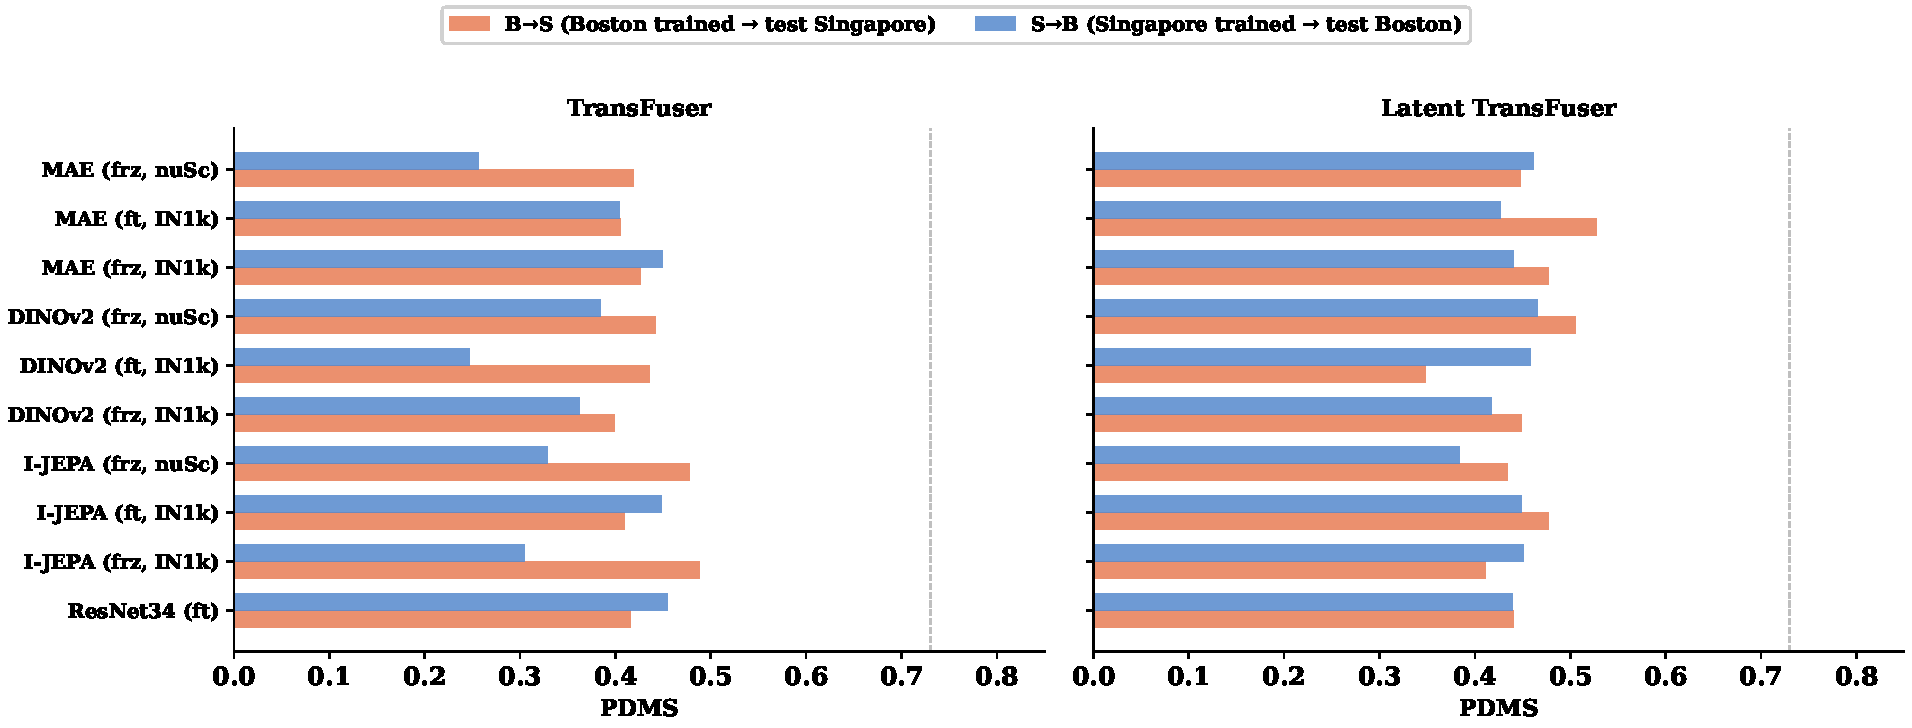
\includegraphics[width=0.78\textwidth]{../fig/iros/fig8_asymmetry.pdf}
  \vspace{4pt}
  \begin{itemize}\footnotesize
    \item Transfer is directional: Boston-to-Singapore is harder than Singapore-to-Boston.
    \item Frozen SSL reduces this asymmetry but does not remove it uniformly across every configuration.
  \end{itemize}
\end{frame}

\begin{frame}{All-city training attenuates backbone differences}
  \centering
  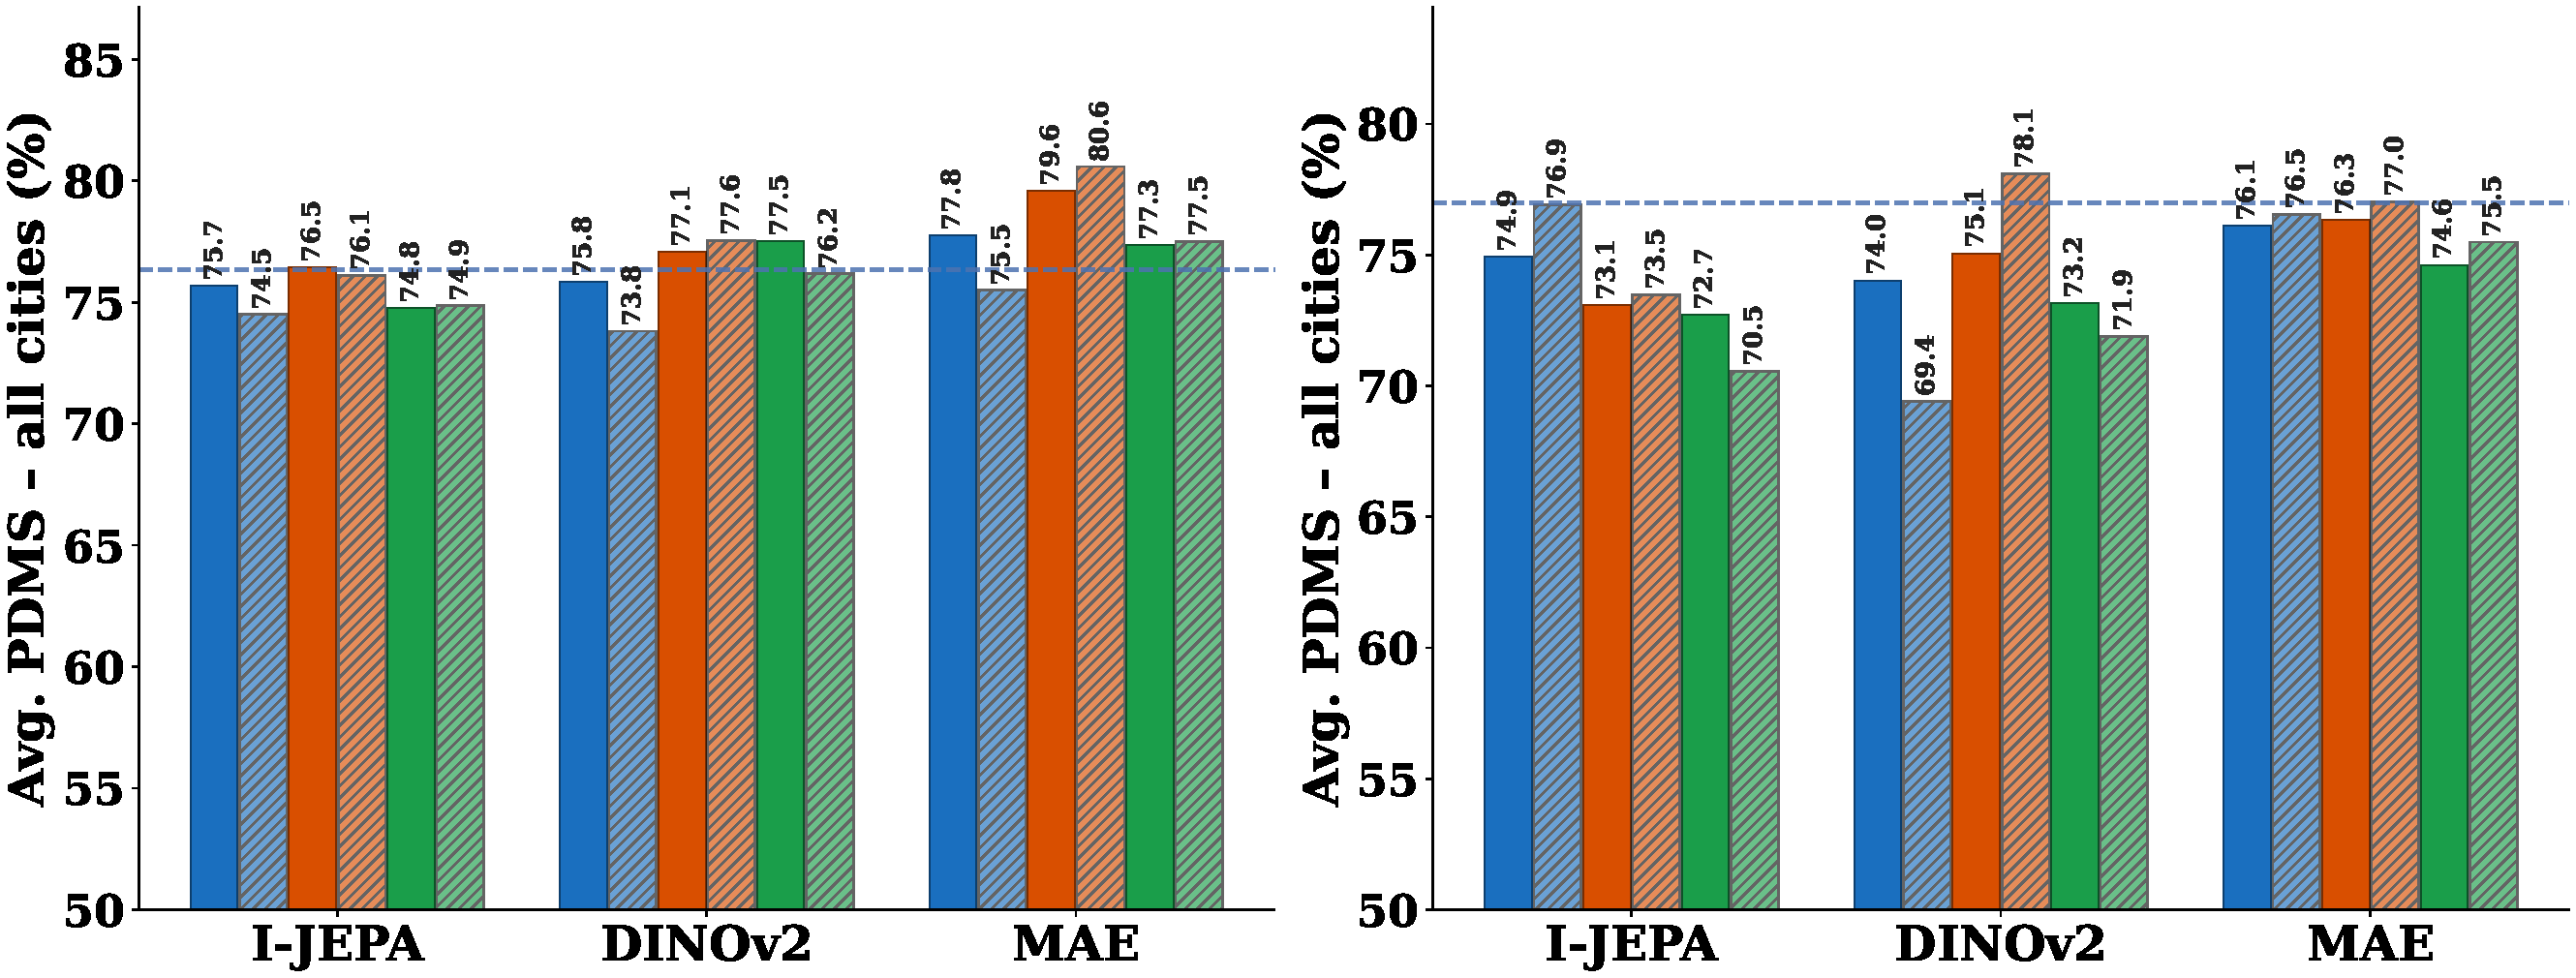
\includegraphics[width=0.78\textwidth]{../fig/iros/fig14_allcity_training.pdf}
  \vspace{4pt}
  \begin{itemize}\footnotesize
    \item Under pooled all-city training, the spread between supervised and SSL backbones shrinks sharply.
    \item This is why the thesis centers city-disjoint transfer rather than mixed-city leaderboard ranking.
  \end{itemize}
\end{frame}

\begin{frame}{Study III: pooled DiffusionDrive results}
  \centering\small
  \textbf{Selected completed rows from pooled NAVSIM}
  \\[4pt]
  \begin{tabular}{@{}l l c c@{}}
    \toprule
    \textbf{Backbone} & \textbf{Modality} & \textbf{Frozen?} & \textbf{PDMS (\%)} \\
    \midrule
    \rowcolor{gray!10}
    \textcolor{sup}{ResNet-34 supervised} & C + L       & --      & $\mathbf{87.9}$ \\
    MAE ViT-S/14 nuSc rect                & C + L       & \cmark  & $86.9$ \\
    MAE ViT-S/14 nuSc sq                  & C + L       & \cmark  & $86.8$ \\
    I-JEPA ViT-S/14 nuSc sq               & C + L       & \cmark  & $86.3$ \\
    \midrule
    \textcolor{sup}{ResNet-34 supervised} & Camera only & --      & $86.6$ \\
    I-JEPA ViT-S/14 nuSc rect             & Camera only & \cmark  & $85.8$ \\
    MAE ViT-S/14 nuSc rect                & Camera only & \cmark  & $83.5$ \\
    \bottomrule
  \end{tabular}
  \vspace{8pt}
  \begin{itemize}\footnotesize
    \item Under pooled evaluation, SSL remains within $1$ to $2$ points of the supervised baseline.
    \item This is the starting point for the city-disjoint DiffusionDrive test.
  \end{itemize}
\end{frame}

\begin{frame}{Study III: cross-city DiffusionDrive transfer}
  \centering
  
\includegraphics[width=0.90\textwidth]{../../navsim-ssl-city-generalization/fig/navsim/dd_cc_interim/dd_cc_transfer_matrix.pdf}
  \vspace{4pt}
  \begin{itemize}\scriptsize
    \item The current thesis record includes Boston-trained and Pittsburgh-trained ResNet-34 rows, and a matched Pittsburgh-trained frozen I-JEPA row.
    \item Across the available rows, Singapore is the weakest destination column.
  \end{itemize}
\end{frame}

\begin{frame}{Study III: matched Pittsburgh comparison}
  \begin{columns}[T]
    \column{0.56\textwidth}
    \centering\scriptsize
    \begin{tabular}{@{}l c c c@{}}
      \toprule
      \textbf{Metric} & \textbf{Rn34-pit} & \textbf{IJSr-pit} & \textbf{Difference} \\
      \midrule
      Pittsburgh in-dist. & $58.0$ & $57.8$ & $-0.2$ \\
      Mean OOD            & $53.5$ & $53.8$ & $+0.3$ \\
      Singapore           & $41.4$ & $43.2$ & $+1.8$ \\
      Pit.\ $\to$ Sin.\ loss & $16.6$ & $14.6$ & $\mathbf{2.0}$ lower \\
      Sin./Pit.\ ratio    & $71.4\%$ & $74.7\%$ & $+3.3$ pts \\
      \bottomrule
    \end{tabular}
    \column{0.44\textwidth}
    \centering\scriptsize
    \begin{tabular}{@{}l c c@{}}
      \toprule
      \textbf{Sub-score} & \textbf{Rn34} & \textbf{IJSr} \\
      \midrule
      NC   & $96.3$ & $96.7$ \\
      DAC  & $61.7$ & $\mathbf{64.1}$ \\
      EP   & $73.7$ & $72.2$ \\
      TTC  & $95.4$ & $96.0$ \\
      Comfort & $0.3$ & $0.5$ \\
      \bottomrule
    \end{tabular}
  \end{columns}
  \vspace{8pt}
  \begin{itemize}\footnotesize
    \item The in-distribution Pittsburgh scores are nearly matched.
    \item The SSL gain is concentrated in drivable-area compliance rather than in collision-adjacent metrics.
  \end{itemize}
\end{frame}

\begin{frame}{Study IV: mechanistic analysis protocol}
  \begin{itemize}
    \item \textbf{Linear city-identification probe.} Measures how much city identity is linearly decodable from the learned features.
    \item \textbf{Effective rank of the feature covariance.} Measures whether the representation collapses onto a small subspace.
    \item \textbf{CKA and MMD.} Auxiliary diagnostics of cross-city similarity and distribution shift.
    \item \textbf{Attention maps.} Qualitative backup only.
  \end{itemize}
  \vspace{6pt}
  \begin{block}{Primary evidence}
    The primary mechanistic evidence in this defense is the training-city-stratified probe pattern, the full-roster summaries, the matched Boston comparison, and the rank contrast between frozen and trainable rows.
  \end{block}
\end{frame}

\begin{frame}{Mechanistic evidence: probe accuracy and OOD loss by training city}
  \centering
  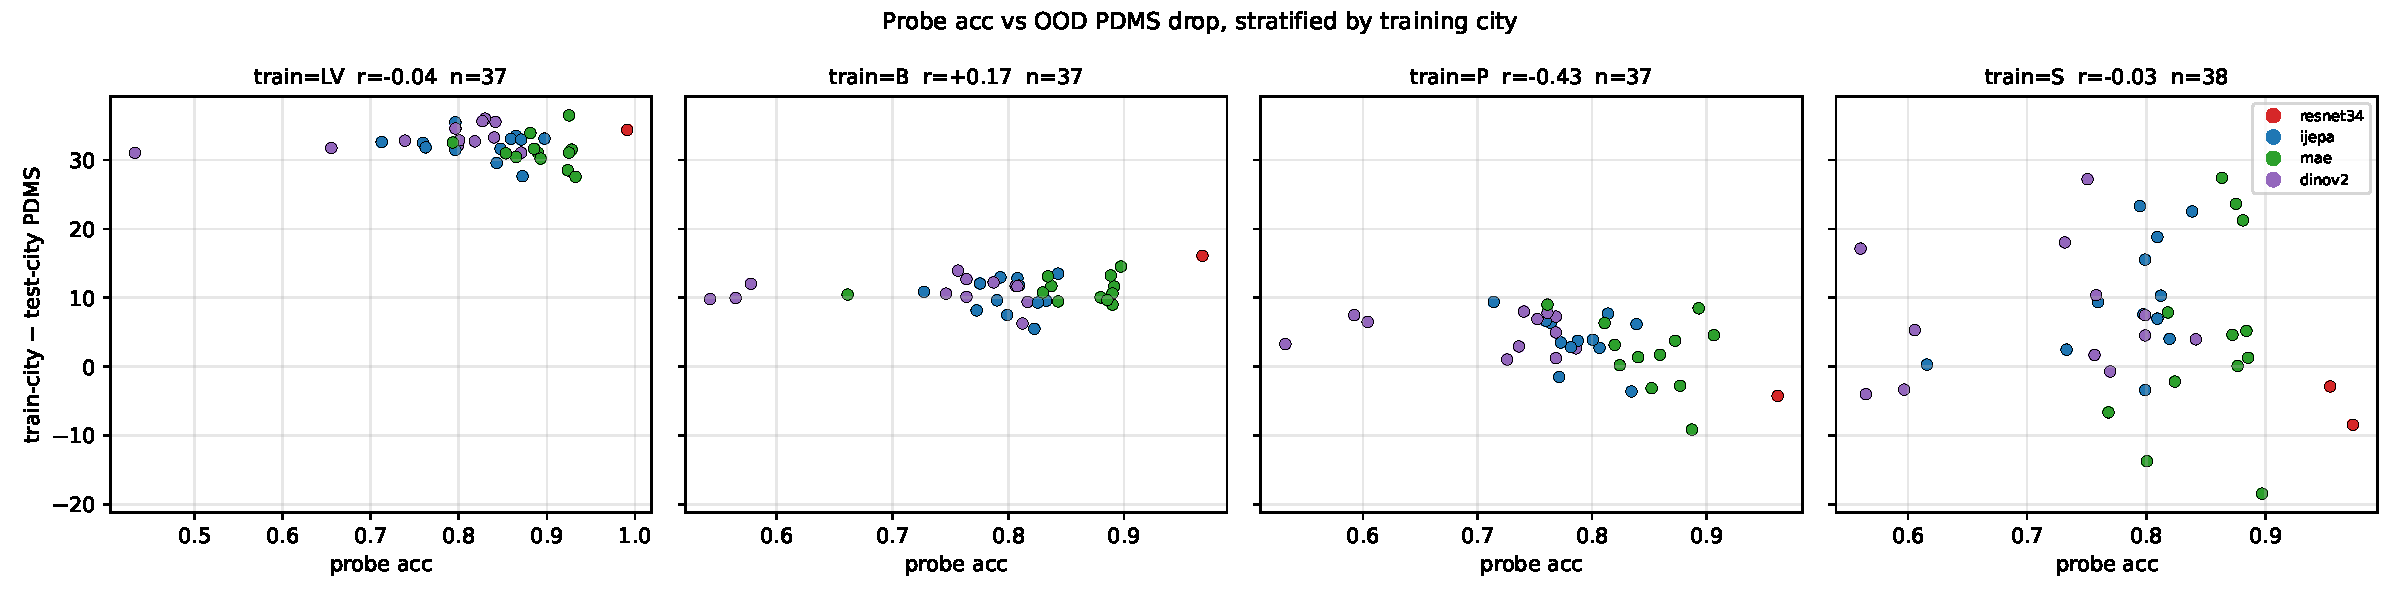
\includegraphics[width=0.92\textwidth]{../fig/phase4/scatter_probe_vs_ood_by_training_city.pdf}
  \vspace{4pt}
  \begin{itemize}\footnotesize
    \item Boston, Pittsburgh, and Las Vegas show the expected upward trend: higher city-decodability corresponds to larger out-of-distribution loss.
    \item Singapore is the exception: the relationship is largely flat in the smallest and most confounded training regime.
  \end{itemize}
\end{frame}

\begin{frame}{Mechanistic evidence: summary across the analysed roster}
  \begin{columns}[T]
    \column{0.51\textwidth}
    \centering
    \textbf{Latent TransFuser}
    \vspace{2pt}
    \scriptsize
    \begin{tabular}{@{}l l c c c@{}}
      \toprule
      \textbf{Family} & \textbf{Status} & \textbf{Probe} & \textbf{Rank} & \textbf{OOD loss} \\
      \midrule
      ResNet-34 & supervised & $0.98$ & $63.3$ & $8.7$ \\
      I-JEPA    & frozen     & $0.83$ & $69.0$ & $11.6$ \\
      I-JEPA    & trainable  & $0.83$ & $46.5$ & $9.5$ \\
      DINOv2    & frozen     & $0.80$ & $58.6$ & $10.0$ \\
      DINOv2    & trainable  & $0.77$ & $65.3$ & $10.0$ \\
      MAE       & frozen     & $0.90$ & $72.6$ & $\mathbf{6.9}$ \\
      MAE       & trainable  & $0.89$ & $49.1$ & $9.2$ \\
      \bottomrule
    \end{tabular}
    \column{0.49\textwidth}
    \centering
    \textbf{TransFuser}
    \vspace{2pt}
    \scriptsize
    \begin{tabular}{@{}l l c c c@{}}
      \toprule
      \textbf{Family} & \textbf{Status} & \textbf{Probe} & \textbf{Rank} & \textbf{OOD loss} \\
      \midrule
      I-JEPA & frozen    & $0.83$ & $66.2$ & $11.4$ \\
      I-JEPA & trainable & $0.75$ & $52.8$ & $12.5$ \\
      DINOv2 & frozen    & $0.74$ & $61.5$ & $12.4$ \\
      DINOv2 & trainable & $0.69$ & $51.6$ & $12.8$ \\
      MAE    & frozen    & $0.89$ & $\mathbf{80.3}$ & $\mathbf{11.2}$ \\
      MAE    & trainable & $0.85$ & $47.5$ & $11.7$ \\
      \bottomrule
    \end{tabular}
  \end{columns}
  \vspace{6pt}
  \footnotesize Values are aggregated across the full analysed roster. The supervised single-city TransFuser row is omitted because the available checkpoint coverage is incomplete.
\end{frame}

\begin{frame}{Mechanistic evidence: matched Boston comparison}
  \centering\small
  \begin{tabular}{@{}l c c c@{}}
    \toprule
    \textbf{Backbone} & \textbf{Probe acc.} & \textbf{OOD mean} & \textbf{OOD loss} \\
    \midrule
    \rowcolor{gray!10}
    \textcolor{sup}{ResNet-34 supervised} & $\mathbf{0.968}$ & $55.6$ & $\mathbf{16.1}$ \\
    MAE ViT-B/16 frozen                   & $0.889$ & $\mathbf{60.2}$ & $13.2$ \\
    I-JEPA ViT-H/14 frozen                & $0.833$ & $57.9$ & $9.6$ \\
    \textcolor{ssl}{DINOv2 ViT-S/14 frozen} & $\mathbf{0.812}$ & $57.3$ & \textbf{6.3} \\
    \bottomrule
  \end{tabular}
  \vspace{8pt}
  \begin{itemize}\footnotesize
    \item This is the identifiable matched comparison used throughout the thesis.
    \item Probe accuracy orders the four backbones the same way as the measured out-of-distribution loss.
  \end{itemize}
\end{frame}

\begin{frame}{Feature-rank collapse under fine-tuning}
  \centering
  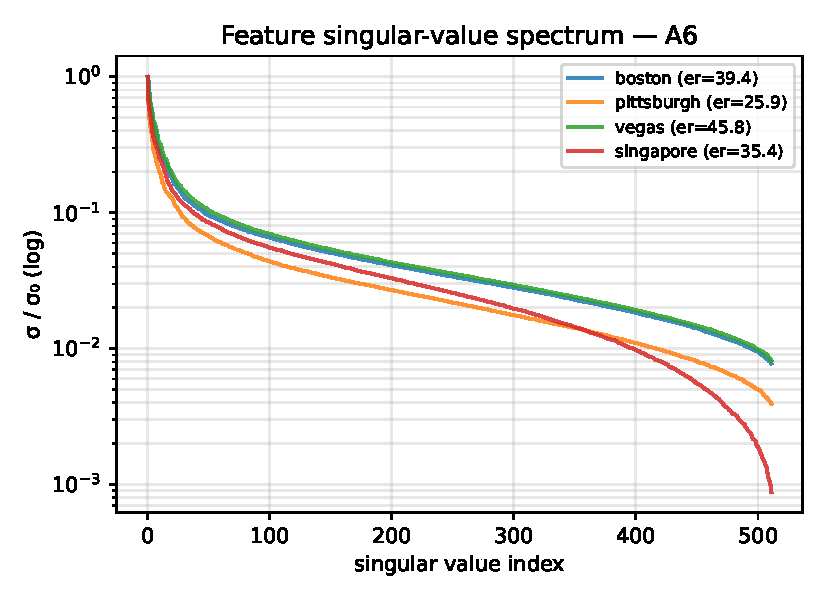
\includegraphics[width=0.44\textwidth]{../fig/phase4/spectrum_A6.pdf}
  \hfill
  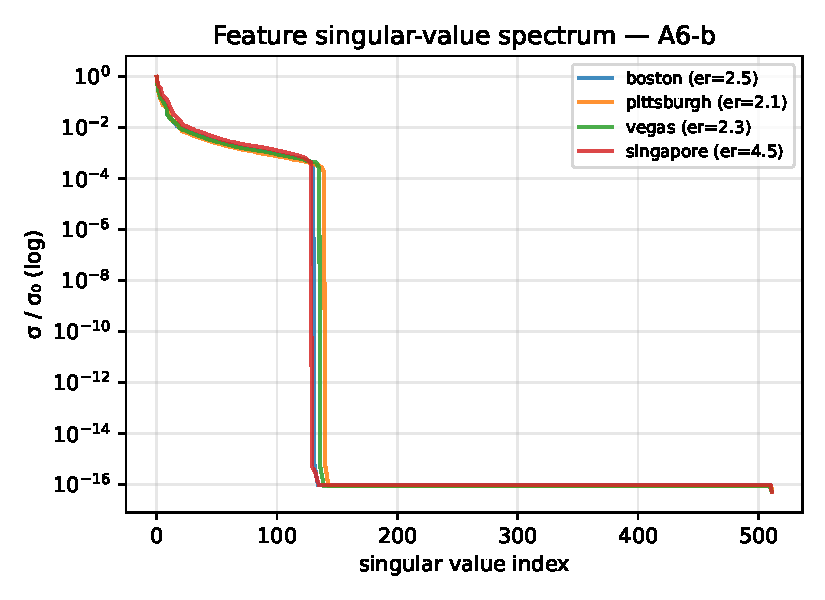
\includegraphics[width=0.44\textwidth]{../fig/phase4/spectrum_A6-b.pdf}
  \vspace{6pt}
  \begin{itemize}\footnotesize
    \item For all-city I-JEPA ViT-H/14, moving from frozen to fully trainable reduces effective rank from $36.6$ to $2.9$ and reduces probe accuracy from $0.94$ to $0.38$.
    \item Fine-tuning can therefore erase useful pretrained structure even when mixed-city fit remains acceptable.
  \end{itemize}
\end{frame}

\section{Discussion}

\sectiondivider{Discussion}

\begin{frame}{Integrated interpretation}
  \begin{enumerate}
    \item Pooled mixed-city metrics underestimate the scale of the representation effect under geographic transfer.
    \item The same signal appears in the lightweight-head study, the LAW benchmark, and the NAVSIM TF and LatTF matrices.
    \item The completed DiffusionDrive rows are directionally consistent with the completed regression-planner results.
    \item The mechanistic evidence supports freezing as an operational choice: transfer degrades when the representation collapses onto city-specific directions.
  \end{enumerate}
\end{frame}

\begin{frame}{Contributions and scope of the claim}
  \begin{columns}[T]
    \column{0.56\textwidth}
    \textbf{Thesis contributions}
    \begin{enumerate}\footnotesize
      \item City-disjoint evaluation on NAVSIM under a validated v1.1 pipeline.
      \item Controlled representation comparisons under LAW, TransFuser, and Latent TransFuser.
      \item DiffusionDrive integration under pooled evaluation and completed cross-city rows.
      \item Mechanistic analysis across the trained-checkpoint roster.
    \end{enumerate}
    \column{0.44\textwidth}
    \textbf{Claim boundary}
    \begin{itemize}\footnotesize
      \item The claim is about representation-mediated geographic transfer.
      \item It is not a claim that planner architecture never matters.
      \item The thesis claim does not depend on a fully populated cross-city DiffusionDrive matrix.
    \end{itemize}
  \end{columns}
\end{frame}

\begin{frame}{Synthesis of the evidence}
  \begin{enumerate}
    \item City-disjoint evaluation exposes a large representation effect that pooled metrics suppress.
    \item Frozen SSL backbones reduce cross-city degradation under both open-loop and closed-loop planners.
    \item The same directional pattern appears in DiffusionDrive on the available cross-city rows.
    \item Mechanistically, better transfer aligns with lower city-decodability in matched settings and with preservation of feature rank under freezing.
  \end{enumerate}
\end{frame}

\begin{frame}{Conclusion}
  \begin{block}{}
    \centering\large
    \textbf{Under city-disjoint evaluation, end-to-end driving failures are strongly mediated by the visual representation. In the evaluated settings, frozen self-supervised backbones transfer more reliably across cities than supervised baselines.}
  \end{block}
  \vspace{10pt}
  \centering
  \textbf{Questions}
\end{frame}

\appendix

\section*{Appendix}

\begin{frame}{A1. Training recipes}
  \centering\scriptsize
  \begin{tabular}{@{}l l l@{}}
    \toprule
    & \textbf{LAW (open-loop, nuScenes)} & \textbf{TF / LatTF (closed-loop, NAVSIM)} \\
    \midrule
    Optimiser      & AdamW                & plain Adam \\
    Base LR        & $5\times10^{-5}$     & $1\times10^{-4}$ constant \\
    Weight decay   & $0.01$               & $0$ \\
    Scheduler      & Cosine to $10^{-3}\!\cdot\!$LR & None \\
    Gradient clip  & $35$                 & $1.0$ \\
    Epochs         & $12$                 & $20$ or $100$ \\
    Batch size     & $2$                  & $32$/GPU, effective $128$ \\
    Hardware       & $1\times$ L40S       & $4\times$ H200 \\
    \bottomrule
  \end{tabular}
  \vspace{6pt}
  \begin{block}{Sensitivity of the TransFuser training recipe}
    \footnotesize Switching to AdamW, adding weight decay, or adding a cosine schedule regresses all-city PDMS sharply. The thesis uses the recipe that reproduces the published TransFuser ordering.
  \end{block}
\end{frame}

\begin{frame}{A2. Freeze and fine-tune details}
  \begin{itemize}
    \item \texttt{trainable\_backbone\_fraction} takes values $0$ or $1$ only.
    \item When unfrozen, encoder parameters use a separate group with LR $3\times10^{-5}$; head LR is $1\times10^{-4}$.
    \item Adapter-side 2-D sin--cos positional encodings are regenerated at the native crop grid.
    \item The planners share a single backbone factory. Changing the backbone is a configuration change, not a model fork.
  \end{itemize}
\end{frame}

\begin{frame}{A3. DiffusionDrive OOD comparison}
  \centering
  \includegraphics[width=0.89\textwidth]{../../navsim-ssl-city-generalization/fig/navsim/dd_cc_interim/dd_cc_ood_drops.pdf}
\end{frame}

\begin{frame}{A4. Full exploratory tables}
  \centering\scriptsize
  \begin{tabular}{@{}l l c c c@{}}
    \toprule
    \textbf{Backbone} & \textbf{Pre-training} & \textbf{P1 (\%)} & \textbf{P3 (\%)} & $\boldsymbol{\Delta}$ \\
    \midrule
    I-JEPA ViT-H/14    & ImageNet-1k SSL           & $79.7$ & $82.5$ & $+2.8$ \\
    MAE ViT-B/16       & ImageNet-1k SSL           & $77.5$ & $\mathbf{84.9}$ & $+7.4$ \\
    MAE ViT-S/14       & nuScenes $224{\times}392$ & $73.8$ & $81.7$ & $+7.9$ \\
    MAE ViT-S/14       & nuScenes $224^2$          & $74.9$ & $81.4$ & $+6.5$ \\
    I-JEPA ViT-S/14    & nuScenes $224^2$          & $71.6$ & $80.9$ & $\mathbf{+9.4}$ \\
    DINOv2 ViT-S/14    & nuScenes $224{\times}392$ & $69.8$ & $76.0$ & $+6.2$ \\
    DINOv2 ViT-S/14    & nuScenes $224^2$          & $69.7$ & $76.0$ & $+6.3$ \\
    \rowcolor{gray!12}
    ResNet-34          & ImageNet supervised       & $68.7$ & $76.9$ & $+8.2$ \\
    DINOv2 ViT-S/14    & LVD-142M SSL              & $66.8$ & $71.8$ & $+5.0$ \\
    I-JEPA ViT-S/14    & nuScenes $224{\times}392$ & $65.4$ & $66.8$ & $+1.4$ \\
    \bottomrule
  \end{tabular}
  \vspace{4pt}
  \footnotesize Pooled \texttt{navtest}, front camera, MLP head, $20$ epochs, AdamW.
\end{frame}

\begin{frame}{A5. Why PDMS remains informative}
  \begin{itemize}
    \item PDMS combines safety, progress, interaction, and comfort on real logged scenarios.
    \item NC and DAC enter multiplicatively, so rare critical failures strongly affect the score.
    \item The thesis treats PDMS as a reproducible proxy and reports changes in out-of-distribution PDMS as the robustness indicator.
    \item Open-loop L2 and collision ratios are reported in parallel on nuScenes.
  \end{itemize}
\end{frame}

\begin{frame}{A6. Baseline validation under NAVSIM v1.1}
  \centering\small
  \begin{tabular}{@{}l c c@{}}
    \toprule
    \textbf{Planner} & \textbf{Published PDMS (\%)} & \textbf{Internal v1.1 PDMS (\%)} \\
    \midrule
    TransFuser & $83.9\pm0.4$ & $83.22$ \\
    Latent TransFuser & $83.5\pm0.6$ & $83.18$ \\
    \bottomrule
  \end{tabular}
  \vspace{8pt}
  \begin{itemize}\footnotesize
    \item Both internal v1.1 runs fall inside the published ranges.
    \item The paper-reported TransFuser and Latent TransFuser ordering is preserved.
    \item This is why the v1.1 cross-city matrix is treated as the canonical thesis record.
  \end{itemize}
\end{frame}

\begin{frame}{A7. Additional Boston-only closed-loop rows}
  \centering\scriptsize
  \begin{tabular}{@{}l c c c c c c@{}}
    \toprule
    \textbf{Boston-only LatTF row} & LV & B & P & S & OOD mean & Loss \\
    \midrule
    ResNet-34 supervised              & $67.3$ & $71.7$ & $54.5$ & $45.0$ & $55.6$ & $16.1$ \\
    MAE ViT-B/16 frozen               & $71.8$ & $73.4$ & $60.0$ & $48.7$ & $60.2$ & $13.2$ \\
    MAE ViT-B/16 trainable            & $69.4$ & $73.1$ & $61.3$ & $53.7$ & $61.5$ & $11.6$ \\
    I-JEPA ViT-H/14 frozen            & $69.4$ & $67.5$ & $62.2$ & $42.2$ & $57.9$ & $9.6$ \\
    I-JEPA ViT-S/14 nuSc rect frozen  & $66.0$ & $68.1$ & $54.9$ & $44.5$ & $55.1$ & $13.0$ \\
    I-JEPA ViT-S/14 nuSc sq frozen    & $71.3$ & $69.6$ & $53.4$ & $48.8$ & $57.8$ & $11.8$ \\
    DINOv2 ViT-S/14 frozen            & $70.7$ & $63.6$ & $55.8$ & $45.5$ & $57.3$ & $6.3$ \\
    DINOv2 ViT-S/14 nuSc rect frozen  & $73.0$ & $69.7$ & $57.3$ & $50.6$ & $60.3$ & $9.4$ \\
    \bottomrule
  \end{tabular}
\end{frame}

\begin{frame}{A8. Linear probe protocol}
  \begin{itemize}
    \item Multinomial logistic regression on standardised backbone features.
    \item Four-way city target: Las Vegas, Boston, Pittsburgh, Singapore.
    \item $80/20$ stratified split on cached features.
    \item Negative control: random-Gaussian features produce probe accuracy $0.254$.
    \item The probe measures linearly decodable city identity; it is not a new planner.
  \end{itemize}
\end{frame}

\begin{frame}{A9. CKA and MMD diagnostics}
  \begin{itemize}
    \item \textbf{CKA} is descriptive: cross-city covariance alignment is high for both supervised and SSL families.
    \item \textbf{MMD\textsuperscript{2}} is an auxiliary diagnostic: useful within matched comparisons, not as a global transfer predictor.
    \item \textbf{Effective rank} is the most interpretable structural measurement for the frozen-versus-trainable contrast.
    \item Attention maps are retained as qualitative backup and are not part of the primary evidence.
  \end{itemize}
\end{frame}

\begin{frame}{A10. Confounders}
  \begin{itemize}
    \item Pretraining domain matters alongside the SSL objective.
    \item Backbone capacity differs across some ImageNet and domain-specific comparisons.
    \item Singapore is confounded by data scale and traffic convention.
    \item Weather, lighting, and season are not independently manipulated.
    \item Seed variance is not measured for the cross-city matrices.
  \end{itemize}
\end{frame}

\begin{frame}{A11. Collaboration and provenance}
  \begin{itemize}
    \item The earlier joint paper is Naeinian, Hamza, Zhu, Choromanska (2026).
    \item LAW and the domain-specific pretraining pipeline come from that collaboration.
    \item This thesis contributes the NAVSIM evaluation pipeline, the planner integrations, the lightweight-head study, and the mechanistic analysis.
  \end{itemize}
\end{frame}

\end{document}
